% ============================================================
% sunum_latex.tex  –  Beamer sunumu (pdflatex)
% HTC VIVE Ultimate Tracker / Alt Ekstremite ROM Analizi
% ============================================================
\documentclass[aspectratio=169,12pt]{beamer}

%% Encoding & language
\usepackage[utf8]{inputenc}
\usepackage[T1]{fontenc}
\usepackage[turkish,shorthands=off]{babel}

%% Math & graphics
\usepackage{amsmath,amssymb}
\usepackage{graphicx}
\usepackage{xcolor}
\usepackage{tikz}
\usepackage{booktabs}
\usepackage{mathptmx}   % Times-like serif

%% Colors
\definecolor{pvred}{HTML}{CF0A2D}
\definecolor{pvnavy}{HTML}{1B2E4A}
\definecolor{pvgray}{HTML}{F4F4F4}

%% ---- Beamer theme ----
\usetheme{default}
\usecolortheme{default}

\setbeamercolor{normal text}{fg=black,bg=white}
\setbeamercolor{frametitle}{bg=pvred,fg=white}
\setbeamercolor{title}{fg=pvnavy}
\setbeamercolor{subtitle}{fg=pvred}
\setbeamercolor{author}{fg=pvnavy}
\setbeamercolor{institute}{fg=black}
\setbeamercolor{date}{fg=pvnavy}
\setbeamercolor{itemize item}{fg=pvred}
\setbeamercolor{itemize subitem}{fg=pvred!70}
\setbeamercolor{enumerate item}{fg=pvred}
\setbeamercolor{block title}{bg=pvred,fg=white}
\setbeamercolor{block body}{bg=pvred!8,fg=black}
\setbeamercolor{footline}{bg=pvnavy,fg=white}
\setbeamercolor{alerted text}{fg=pvred}

\setbeamerfont{frametitle}{series=\bfseries,size=\large}
\setbeamerfont{title}{series=\bfseries,size=\Large}
\setbeamerfont{subtitle}{series=\mdseries,size=\normalsize}
\setbeamerfont{footline}{size=\scriptsize}

\setbeamertemplate{navigation symbols}{}
\setbeamertemplate{itemize item}{\small\textbullet}
\setbeamertemplate{itemize subitem}{--}

%% Thin red top rule on each content slide
\setbeamertemplate{headline}{%
  \begin{beamercolorbox}[wd=\paperwidth,ht=1.5pt]{frametitle}%
  \end{beamercolorbox}%
}

%% Frametitle bar
\setbeamertemplate{frametitle}{%
  \begin{beamercolorbox}[wd=\paperwidth,ht=0.72cm,dp=0.12cm,leftskip=0.55cm]{frametitle}%
    \usebeamerfont{frametitle}\insertframetitle%
  \end{beamercolorbox}%
}

%% Footline
\setbeamertemplate{footline}{%
  \begin{beamercolorbox}[wd=\paperwidth,ht=0.42cm,dp=0.18cm,leftskip=0.45cm,rightskip=0.45cm]{footline}%
    G\"{u}m\"{u}\c{s}hane \"{U}niversitesi
    \(\cdot\) Yaz\i{}l\i{}m M\"{u}hendisli\u{g}i
    \(\cdot\) 2026%
    \hfill%
    \insertframenumber/\inserttotalframenumber%
  \end{beamercolorbox}%
}

\graphicspath{{./}}
\setlength{\itemsep}{0.3em}

% ============================================================
\begin{document}
% ============================================================

%% ============================================================
%% Slayt 1 – Kapak
%% ============================================================
{%
\setbeamertemplate{headline}{}
\setbeamertemplate{footline}{}
\begin{frame}[noframenumbering,plain]
  \begin{tikzpicture}[remember picture,overlay]
    % Left red stripe
    \fill[pvred] (current page.north west)
                 rectangle ([xshift=0.55cm]current page.south west);
    % Top navy band
    \fill[pvnavy] ([xshift=0.55cm]current page.north west)
                  rectangle ([yshift=-0.65cm]current page.north east);
    % Bottom navy band
    \fill[pvnavy] (current page.south west)
                  rectangle ([yshift=0.50cm]current page.south east);
    % Red corner accent – top right
    \fill[pvred] ([xshift=-2.0cm]current page.north east)
                 rectangle ([yshift=-0.65cm]current page.north east);
  \end{tikzpicture}
  \vspace{1.1cm}
  \begin{center}
    {\color{pvred}\textbf{\large L\.{I}SANS B\.{I}T\.{I}RME PROJES\.{I}}}\\[0.55em]
    {\color{pvnavy}\textbf{\large
      HTC VIVE Ultimate Tracker ve XR Tabanl\i{}\\[0.2em]
      Oyunla\c{s}t\i{}r\i{}lm\i{}\c{s} Alt Ekstremite Hareket Analizi Sistemi}}\\[0.8em]
    {\large Muhammet \c{C}i\u{g}dem \quad\(\cdot\)\quad 227231041}\\[0.3em]
    {Dan\i{}\c{s}man: Dr.\ \"{O}\u{g}r.\ \"{U}yesi Samet Tonyal\i{}}\\[0.55em]
    {\color{pvnavy}\itshape
      G\"{u}m\"{u}\c{s}hane \"{U}niversitesi \(\cdot\)
      Yaz\i{}l\i{}m M\"{u}hendisli\u{g}i \(\cdot\) May\i{}s 2026}
  \end{center}
\end{frame}
}

%% ============================================================
%% Slayt 2 – Problem ve Motivasyon
%% ============================================================
\begin{frame}{Problem ve Motivasyon}
  \begin{itemize}\setlength\itemsep{0.35em}
    \item Diz valgusu, tek ayak dengesizli\u{g}i ve y\"{u}k kabul\"{u} gibi dinamik paternler
          statik a\c{c}\i{} \"{o}l\c{c}\"{u}mleriyle yeterince a\c{c}\i{}klanamaz.
    \item Laboratuvar tipi hareket yakalama sistemleri pahal\i{} ve
          ta\c{s}\i{}nabilirli\u{g}i s\i{}n\i{}rl\i{}d\i{}r.
    \item Geleneksel gonyometri de\u{g}erlendirici ba\u{g}\i{}ml\i{}d\i{}r ve
          anl\i{}k \"{o}l\c{c}\"{u}m s\i{}n\i{}rl\i{}l\i{}klar\i{} ta\c{s}\i{}r.
  \end{itemize}

  \vspace{0.6em}
  \textcolor{pvred}{\textbf{Hedef}}
  \begin{itemize}\setlength\itemsep{0.3em}
    \item HTC VIVE Ultimate Tracker + OpenXR ile eri\c{s}ilebilir bir altyap\i{} kurmak,
    \item G\"{o}rev tabanl\i{} bir XR ak\i{}\c{s}\i{}na d\"{o}n\"{u}\c{s}t\"{u}rmek,
    \item Tan\i{} iddias\i{} ta\c{s}\i{}mayan destekleyici hareket tarama
          \c{c}\i{}kt\i{}lar\i{} \"{u}retmek.
  \end{itemize}
\end{frame}

%% ============================================================
%% Slayt 3 – Sistem Mimarisi ve Yöntem
%% ============================================================
\begin{frame}{Sistem Mimarisi ve Y\"{o}ntem}
  \begin{columns}[T]
    \begin{column}{0.58\textwidth}
      \textcolor{pvred}{\textbf{Donan\i{}m \& Yaz\i{}l\i{}m}}
      \begin{itemize}\setlength\itemsep{0.25em}
        \item HTC VIVE Ultimate Tracker: pelvis, femur, tibia --
              ihtiya\c{c} h\^{a}linde \"{u}st ekstremite.
        \item Unity~6, OpenXR ve VIVE eklentileri; FK + IK \c{c}\"{o}z\"{u}c\"{u}ler.
      \end{itemize}

      \vspace{0.5em}
      \textcolor{pvred}{\textbf{4 Katmanl\i{} Veri Ak\i{}\c{s}\i{}}}
      \begin{itemize}\setlength\itemsep{0.25em}
        \item OpenXR Cihaz Katman\i{} $\rightarrow$ Toplama ve E\c{s}leme Katman\i{}
        \item Kinematik \c{C}\"{o}z\"{u}m (FK + tam v\"{u}cut IK) $\rightarrow$
              Uygulama (g\"{o}rev motoru, UI, raporlama)
      \end{itemize}
    \end{column}

    \begin{column}{0.38\textwidth}
      \begin{block}{Kalibrasyon}
        \[Q_{offset} = Q_T^{-1} \cdot Q_B\]
        \vspace{-0.4em}
        \c{C}al\i{}\c{s}ma an\i{}:
        \[Q_B(t) = Q_T(t) \cdot Q_{offset}\]
      \end{block}
      \vspace{0.35em}
      \small Kalibrasyon bazl\i{} sens\"{o}r-kemik ofseti FK hiyerar\c{s}isi
      \"{u}zerinden uygulan\i{}r.
    \end{column}
  \end{columns}
\end{frame}

%% ============================================================
%% Slayt 4 – Görevler ve Üretilen Metrikler
%% ============================================================
\begin{frame}{G\"{o}revler ve \"{U}retilen Metrikler}
  \begin{columns}[T]
    \begin{column}{0.56\textwidth}
      \begin{itemize}\setlength\itemsep{0.22em}
        \item Kontroll\"{u} ini\c{s} $\rightarrow$
              pik diz valgusu \(\cdot\) diz fleksiyonu \(\cdot\) sway
        \item Mini squat $\rightarrow$
              diz fleksiyonu \(\cdot\) valgus e\u{g}ilimi
        \item Tek ayak squat (sa\u{g}/sol) $\rightarrow$
              diz valgusu \(\cdot\) fleksiyon \(\cdot\) sway
        \item Mod.\ anterior reach (sa\u{g}/sol) $\rightarrow$
              reach\,\% \(\cdot\) stance valgusu \(\cdot\) sway
        \item Tek ayak denge (sa\u{g}/sol) $\rightarrow$
              pelvis sway RMS \(\cdot\) sway h\i{}z\i{}
        \item G\"{o}vde e\u{g}imi \& yerinde y\"{u}r\"{u}me $\rightarrow$
              proksimal kontrol
      \end{itemize}
    \end{column}

    \begin{column}{0.40\textwidth}
      \begin{block}{Form\"{u}ller}
        \[\mathrm{Reach\,\%} = \dfrac{d_{\mathrm{reach}}}{L_{\mathrm{limb}}} \times 100\]
        \[\mathrm{Sway_{RMS}} = \sqrt{\dfrac{1}{N}\sum_{i}(x_i - \bar{x})^2}\]
      \end{block}
      \vspace{0.4em}
      \small Sonu\c{c}lar T\"{u}rk\c{c}e yorum ve risk alan\i{} bild\i{}r\i{}mine
      d\"{o}n\"{u}\c{s}t\"{u}r\"{u}lmektedir.
    \end{column}
  \end{columns}
\end{frame}

%% ============================================================
%% Slayt 5 – Bulgular ve Görsel Anlatım
%% ============================================================
\begin{frame}{Bulgular ve G\"{o}rsel Anlat\i{}m}
  \begin{columns}[T]
    \begin{column}{0.54\textwidth}
      \centering
      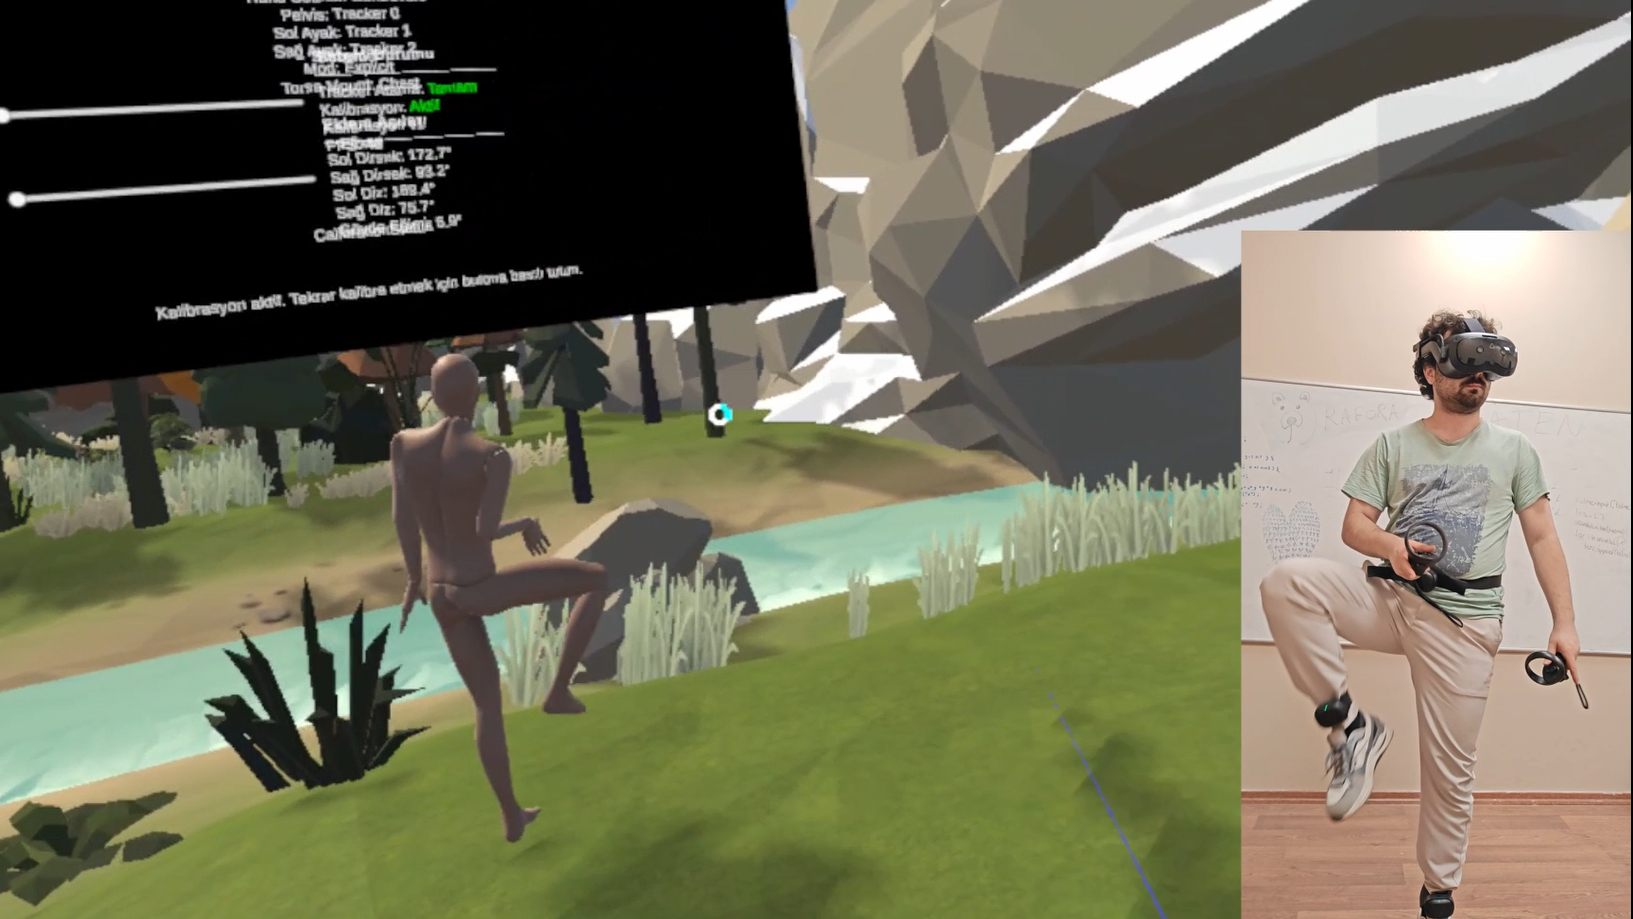
\includegraphics[width=\linewidth]{oyun_ici.png}
    \end{column}

    \begin{column}{0.43\textwidth}
      \vspace{0.4em}
      \textcolor{pvred}{\textbf{Bulgular}}
      \begin{itemize}\setlength\itemsep{0.55em}
        \item Tracker verisinden ger\c{c}ek zamanl\i{}
              kalca/diz kinemati\u{g}i \"{u}retimi.
        \item E\c{s}zamanl\i{} tam v\"{u}cut avatar
              s\"{u}r\"{u}\c{s}\"{u} ve g\"{o}rsel geri bildirim.
        \item G\"{o}rev tabanl\i{}, yorumlanabilir
              metrik ak\i{}\c{s}\i{}.
        \item Hint d\"{u}zeltmesi, bind-pose s\i{}f\i{}rla\-ma ve
              shin-tracker temsili.
      \end{itemize}
    \end{column}
  \end{columns}
\end{frame}

%% ============================================================
%% Slayt 6 – Teknik Görseller
%% ============================================================
\begin{frame}{Teknik G\"{o}rseller}
  \begin{columns}[T,totalwidth=\textwidth]
    \begin{column}{0.31\textwidth}
      \centering
      \includegraphics[width=\linewidth,height=5.8cm,keepaspectratio]%
        {tracker_yerlesim.jpg}\\[0.15em]
      {\small\color{pvnavy} Tracker Yerle\c{s}imleri}
    \end{column}

    \begin{column}{0.02\textwidth}\end{column}

    \begin{column}{0.31\textwidth}
      \centering
      \includegraphics[width=\linewidth,height=5.8cm,keepaspectratio]%
        {editor_oyun.png}\\[0.15em]
      {\small\color{pvnavy} Edit\"{o}r -- Oyun \.{I}\c{c}i G\"{o}r\"{u}nt\"{u}}
    \end{column}

    \begin{column}{0.02\textwidth}\end{column}

    \begin{column}{0.31\textwidth}
      \centering
      \includegraphics[width=\linewidth,height=5.8cm,keepaspectratio]%
        {kayit_analiz.png}\\[0.15em]
      {\small\color{pvnavy} Kay\i{}t Analizi}
    \end{column}
  \end{columns}
\end{frame}

%% ============================================================
%% Slayt 7 – Sınırlılıklar ve Sonuç
%% ============================================================
\begin{frame}[shrink=8]{S\i{}n\i{}rl\i{}l\i{}klar, Gelecek \c{C}al\i{}\c{s}malar ve Sonu\c{c}}
  \begin{columns}[T]
    \begin{column}{0.48\textwidth}
      \textcolor{pvred}{\textbf{S\i{}n\i{}rl\i{}l\i{}klar}}
      \begin{itemize}\setlength\itemsep{0.15em}
        \item Referans sistemle nicel do\u{g}rulama hen\"{u}z yap\i{}lmam\i{}\c{s}t\i{}r.
        \item G\"{o}revler LESS / Y-Balance ile bire bir e\c{s}le\c{s}memektedir.
        \item Trunk lean ve y\"{u}r\"{u}me sim\"{u}lasyonu klinik
              \"{o}l\c{c}\"{u}t \"{u}retmemektedir.
      \end{itemize}

      \vspace{0.3em}
      \textcolor{pvred}{\textbf{Gelecek \c{C}al\i{}\c{s}malar}}
      \begin{itemize}\setlength\itemsep{0.15em}
        \item Klinik gonyometre / referans sistemle ROM do\u{g}rulamas\i{}.
        \item Y\"{u}r\"{u}y\"{u}\c{s} ve trunk metriklerinin eklenmesi.
        \item Terapist paneli ve raporlama mod\"{u}l\"{u}.
      \end{itemize}
    \end{column}

    \begin{column}{0.48\textwidth}
      \begin{block}{Sonu\c{c}}
        \small ROM \"{o}l\c{c}\"{u}m\"{u}, full-body avatar s\"{u}r\"{u}\c{s}\"{u} ve
        oyunla\c{s}t\i{}r\i{}lm\i{}\c{s} g\"{o}rev ak\i{}\c{s}\i{} tek mimaride
        birle\c{s}tirilerek savunulabilir bir lisans bitirme prototipi sunulmu\c{s}tur.
      \end{block}
      \vspace{0.15em}
      \scriptsize Mevcut \c{c}\i{}kt\i{} tan\i{} ama\c{c}l\i{} de\u{g}ildir.
      Klinik ge\c{c}erlilik i\c{c}in uzman g\"{o}r\"{u}\c{s}\"{u} ve referans
      sistem do\u{g}rulamas\i{} \"{o}nerilmektedir.
    \end{column}
  \end{columns}
\end{frame}

\end{document}
